%
% Section The Stroboscopic Approach}
%
\section{The Stroboscopic Approach}
\label{approach}
We have dubbed the time-slicing of neutrino events relative to the
time of their parent bunch as a 'stroboscopic' approach, as it is
essentially successive snapshots of the neutrino bunch but with
different energy spectra and different neutrino family populations in
each time bin. We describe the basic ingredients of the technique
below.

\subsection{Timing Relative to Wave Fronts of Zero Time At the Detector}
\label{wave_front}

The 53-MHz RF structure of the proton beam at the neutrino target imprints
the interaction rate on the production of the hadrons that are the
primary source of neutrinos, as indicated in
Figure~\ref{fig:wave_fronts}. The spacing of the resulting neutrino bunches is given by the
period of the RF structure on the proton beam, $\tau$. The length of
the neutrino bunch depends on both the proton bunch length, convoluted with the difference in time between the
production of the parent hadrons  at the target, and their subsequent
decay that produces the neutrinos. An additional factor is the
different path lengths of the parent hadrons through the neutrino
focusing horn and decay region. 

\begin{figure}[ht]
	\begin{center}
           	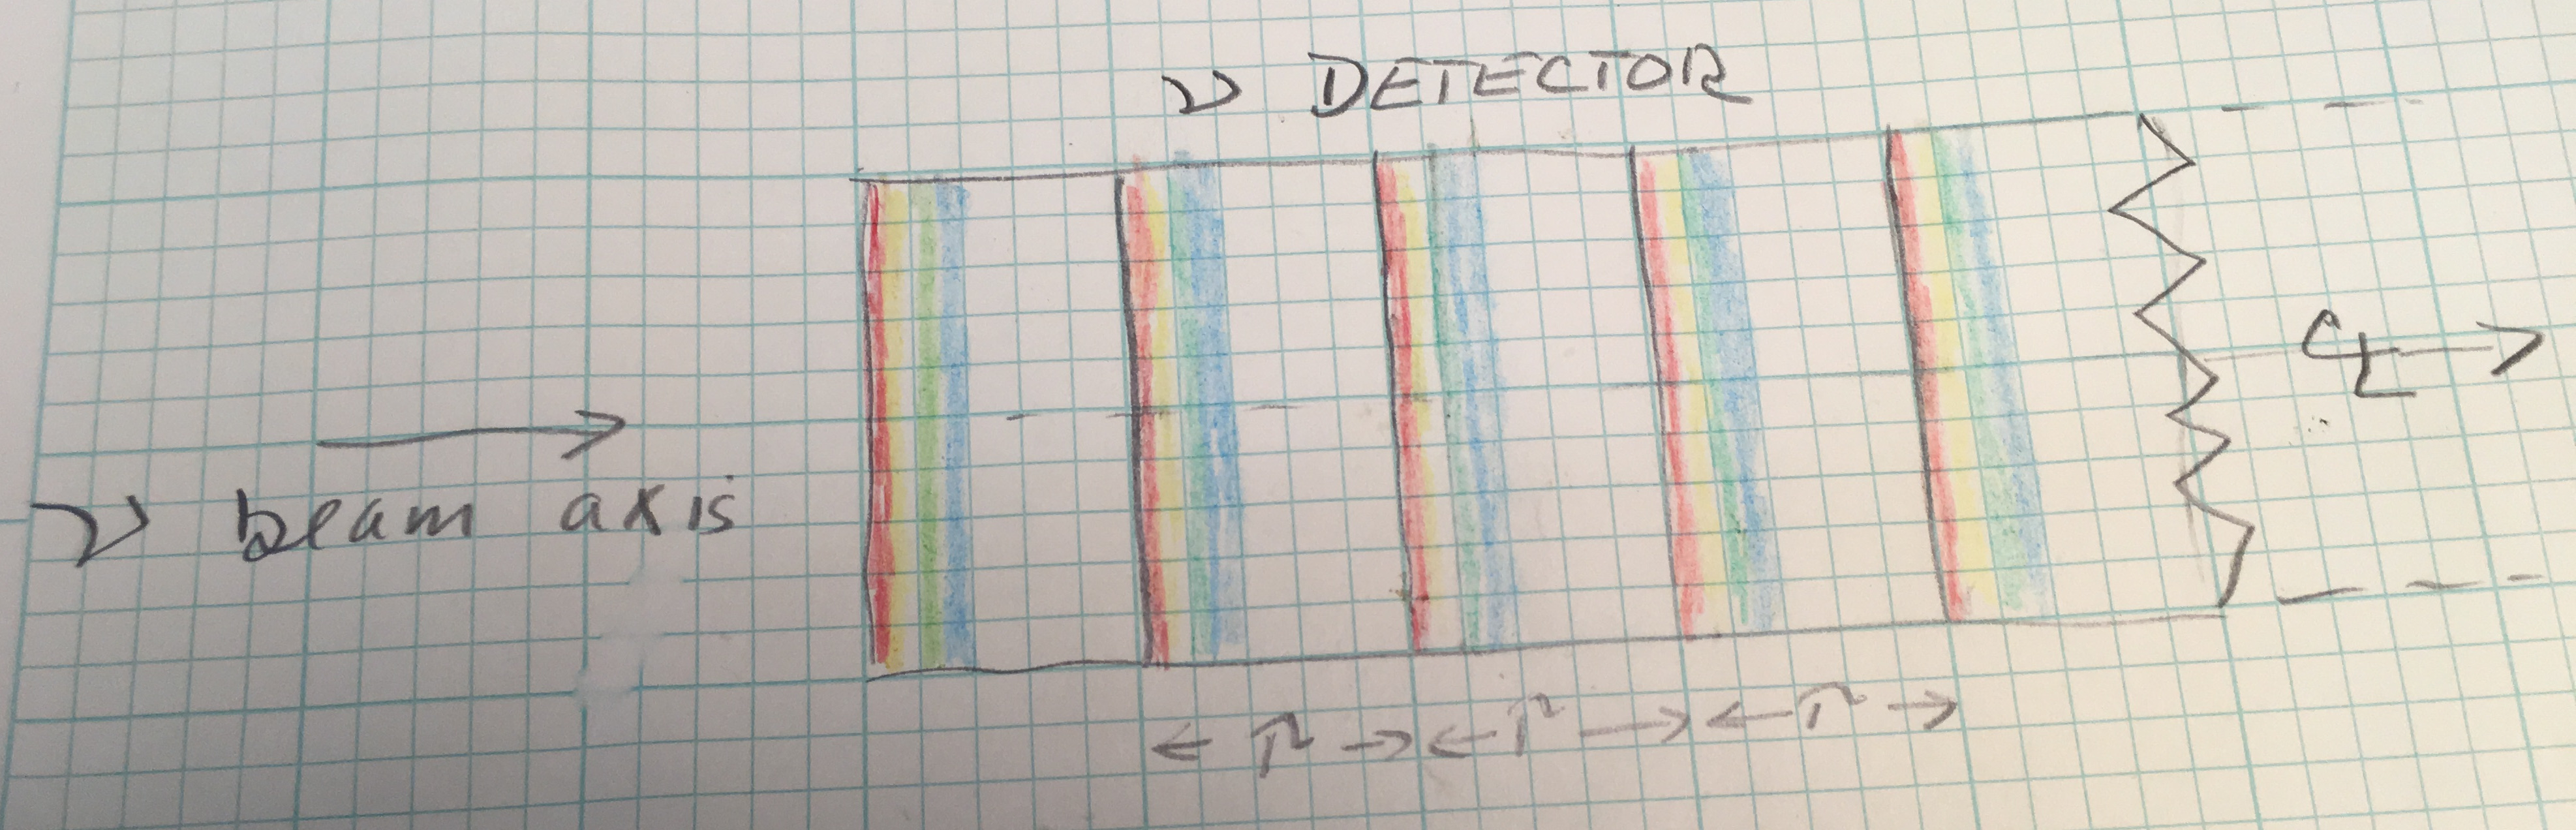
\includegraphics[width=1.0 %\linewidth]{Figures/nupaper_waves_IMG_5834_crop.jpg}
           	   \linewidth]{Figures/NeutrinoBunches.png}
	\end{center}
	\caption{A `snap-shot' of the neutrino wave-front moving
          through a neutrino detector.}

	\label{fig:wave_fronts}
\end{figure}



\subsection{Time Reference to Proton Bunch-by-Bunch Interaction
  Profiles at the Target}
\label{time_reference}

Figure~\ref{fig:bucket_timing} shows the time relationship between the
RF bunch structure of the protons at the target and the neutrino events in a
detector at distance L from the target. The period of the RF is
denoted by $\tau$, and the FWHM of the proton bunch is denoted by
$\sigma_p$. Each neutrino bunch is offset to a later time from its
parent proton bunch by approximately $L/c$, where $c$ is the speed of
light.

The neutrinos from a given proton bunch arrive at the detector before
a signal can be transmitted using electromagnetism, i.e. real or
virtual photons. One consequently has to locally record the relevant
data on a bunch-to-bunch basis at the RF frequency. Each bunch should be
time stamped at both the target and the detector so that the data from
target and detector can be re-united robustly. Section~\ref{muon_monitor} describes the muon monitor
systems that provide the data on the time profile of protons on target
for each bunch. 

\begin{figure}[ht]
	\begin{center}
           	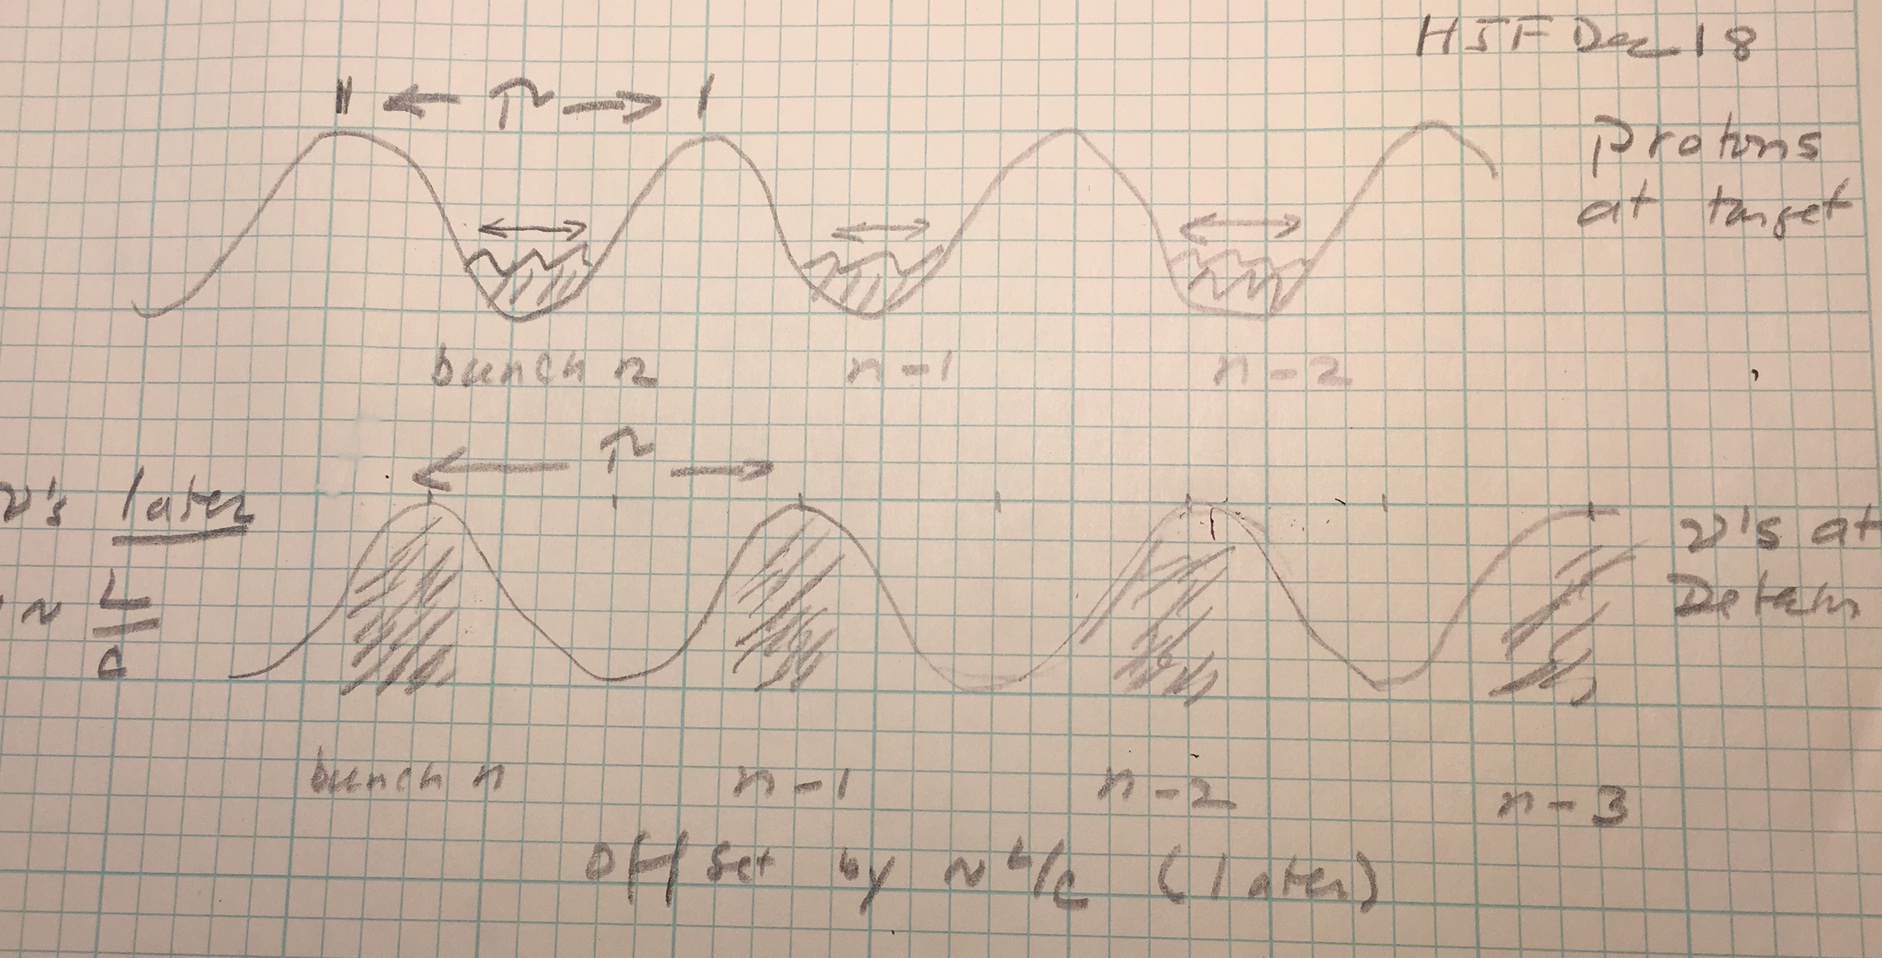
\includegraphics[width=0.7 \linewidth]{Figures/nupaper_timing_IMG_5836_crop.jpg}
	\end{center}
	\caption{A 'cartoon' of the correspondence bucket-by-bucket of
          the neutrino neutrino wave-front timing at the neutrino
          detector and the protons interacting with the target. The
          separation is given by the RF period $\tau$, and the FWHM of
        the proton bunch is denoted by $\sigma_p$.}
	\label{fig:bucket_timing}
\end{figure}

\subsection{Energy and Flavor Spectra Sorted by Time Slice Relative to the Parent Proton Bunch}
\label{spectra}


Figure~\ref{fig:wave_fronts} also indicates the `stroboscopic' nature of this proposal. Neutrinos from lower energy hadron parents (indicated in red) arrive in a distribution that tends later than neutrinos from higher energy
parents (indicated in blue), as described below in Section~\ref{mechanism}. Time-slicing relative to the specific parent proton  bunch, i.e. on a bunch-to-bunch basis, produces different energy spectra in each
time-slice. The spectra will also depend on the family type of the
neutrino, as electrons and muons are produced in different rations
from pions and kaons, and tau neutrinos, while rare, will be
predominantly produced by short-lived parents.

To illustrate the potential value of this approach, the left panel of Fig~\ref{fig:timeslices1} shows the simulated beam energy spectrum for different selection cuts with respect to the start time of the neutrino bunch in Forward Horn Current (FHC) operation of the LBNF beam. Similarly, the right panel Fig~\ref{fig:timeslices1} shows the fractional composition of the different sign and flavor components of the bem in Reverse Horn Current (RHC) mode. 

The ability to use timing to select different flavor and energy components of the neutrino beam will provide a strong  handle for controlling beam and cross section systematics, understanding and controlling backgrounds, and demonstrating the robustness of oscillation measurements.

\begin{figure}[t]
	\begin{center}
        	\begin{tabular}{c c}
        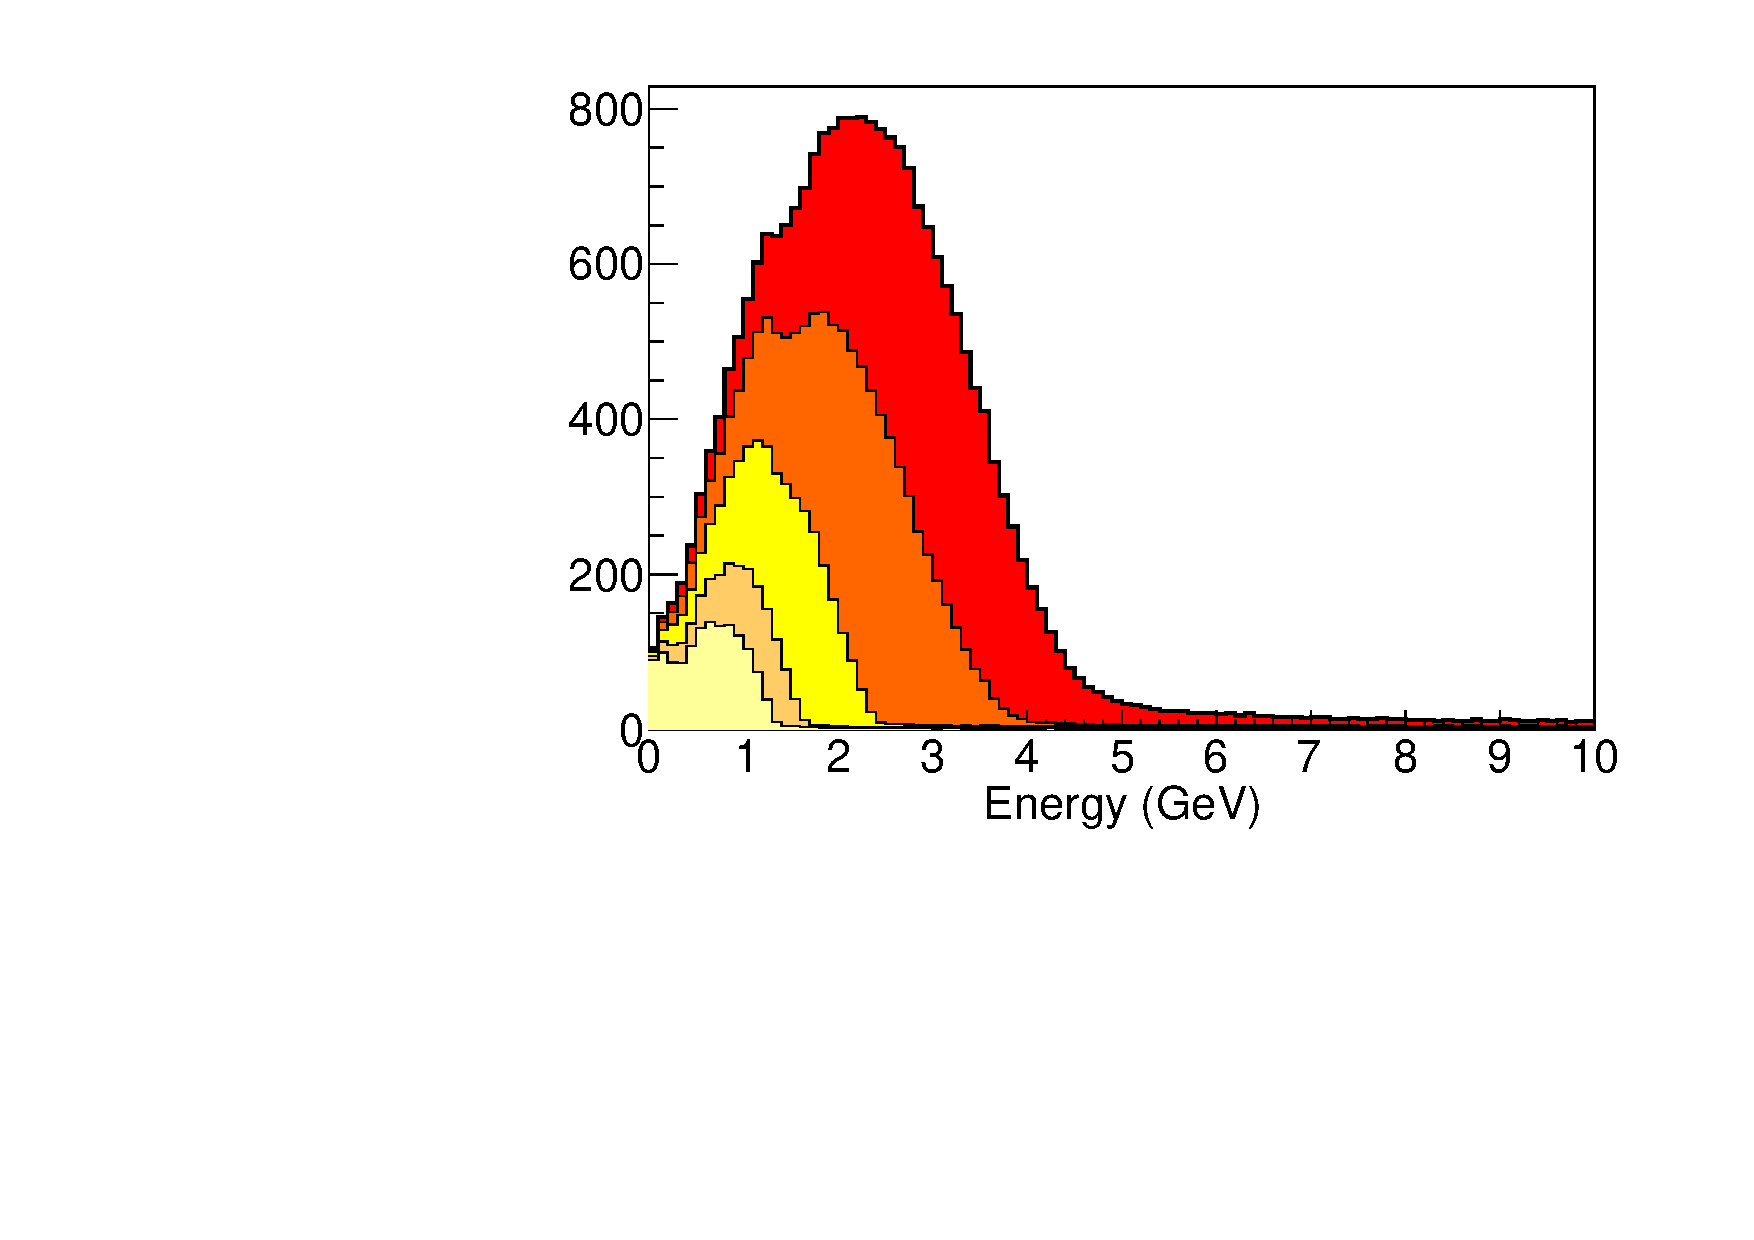
\includegraphics[width=0.5\linewidth]{Figures/DUNEbeam_truetimingB.pdf} &
        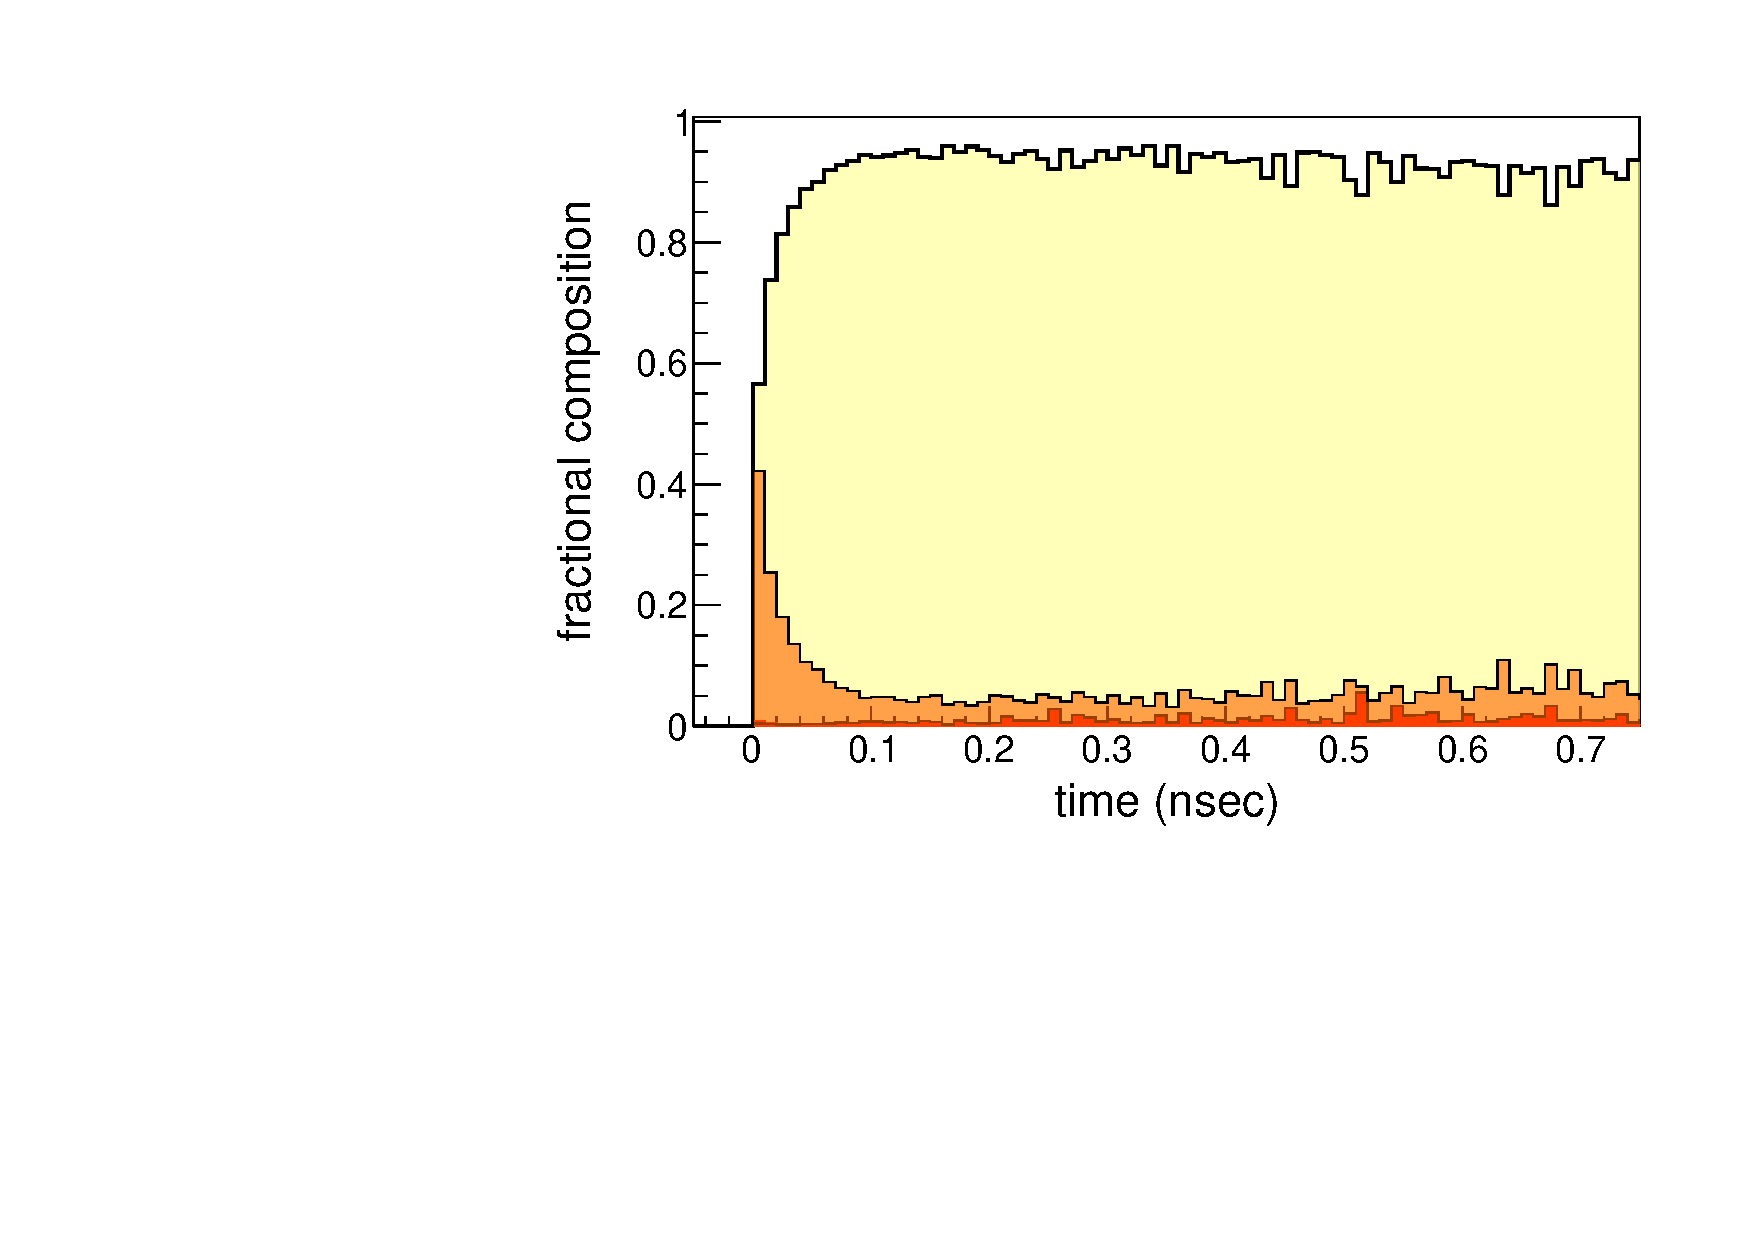
\includegraphics[width=0.5\linewidth]{Figures/wrongsigncomposition_RHC.pdf} \\
	\end{tabular}
	\end{center}
	\caption{LEFT: The simulated  DUNE forward horn current flux (red), with the
          fluxes corresponding to increasingly later time-cuts on the
          bunch time, assuming no time spread of the protons on
          target: 250 psec after the start of the neutrino bunch
          (orange), 500 psec after (yellow), 750 psec (dark beige), 1
          nsec (light beige). RIGHT: The fractional composition of the beam in reverse horn current as a function of time, for muon antineutrinos (light yellow), wrong-sign contributions of muon neutrinos (orange), and electron neutrinos (red). }
		\label{fig:timeslices1}
\end{figure}

\subsection{Derrivation of the Effect}
\label{mechanism}

The difference in arrival time of a neutrino from a sub-relativistic
pion of energy E' with respect to a high energy pion traveling with
speed $\sim$c is given by:

\begin{equation}
\Delta t(E') = \frac{c - v(E')}{c} \tau (E')
\end{equation}

Where $\tau (E')$ is the lifetime of the lower energy pion in the lab
frame. The time spreading will only occur until the decay of the lower
energy pion, at which point the daughter neutrinos will propagate at
c. The lifetime of the higher energy pion is irrelevant, since the
pion is already propagating at roughly c.

\begin{equation}
\Delta t(E') = \tau (E') [1 - \beta (E')]
\end{equation}

Rewriting in terms of the pion lifetime in the restframe, $\tau_0$, we get:

\begin{equation}
\Delta t(E') = \left(\frac{E'}{m} \tau_0\right) \left[1 - \sqrt{ 1 - \frac{m^2}{E'^2}} \right] 
\end{equation}

Regrouping the equation, we get the relationship:

\begin{equation}
\Delta t(E') = \left[\frac{E'}{m} - \sqrt{ \frac{E'^2}{m^2} - 1}\right] \tau_0
\label{eq:beamkinematicsandtiming}
\end{equation}

As one would expect, at the lowest energies, where the pion is
essentially at rest in the lab frame, $\Delta t(E')$ approaches the
lifetime of the pion in the rest frame, $\tau_0$. At high energies,
the speed of the lower-energy pion approaches that of the higher
energy pion and thus $\Delta t(E')$ goes to zero.

Figure~\ref{fig:beamkinematicsandtiming} shows a plot of
equation~\ref{eq:beamkinematicsandtiming} (TOP), and the simulated
relationship between $\Delta t(E')$ and E' for the DUNE beam.

\begin{figure}[h]
	\begin{center}
           	\begin{tabular}{c c}
 \multicolumn{2}{c}{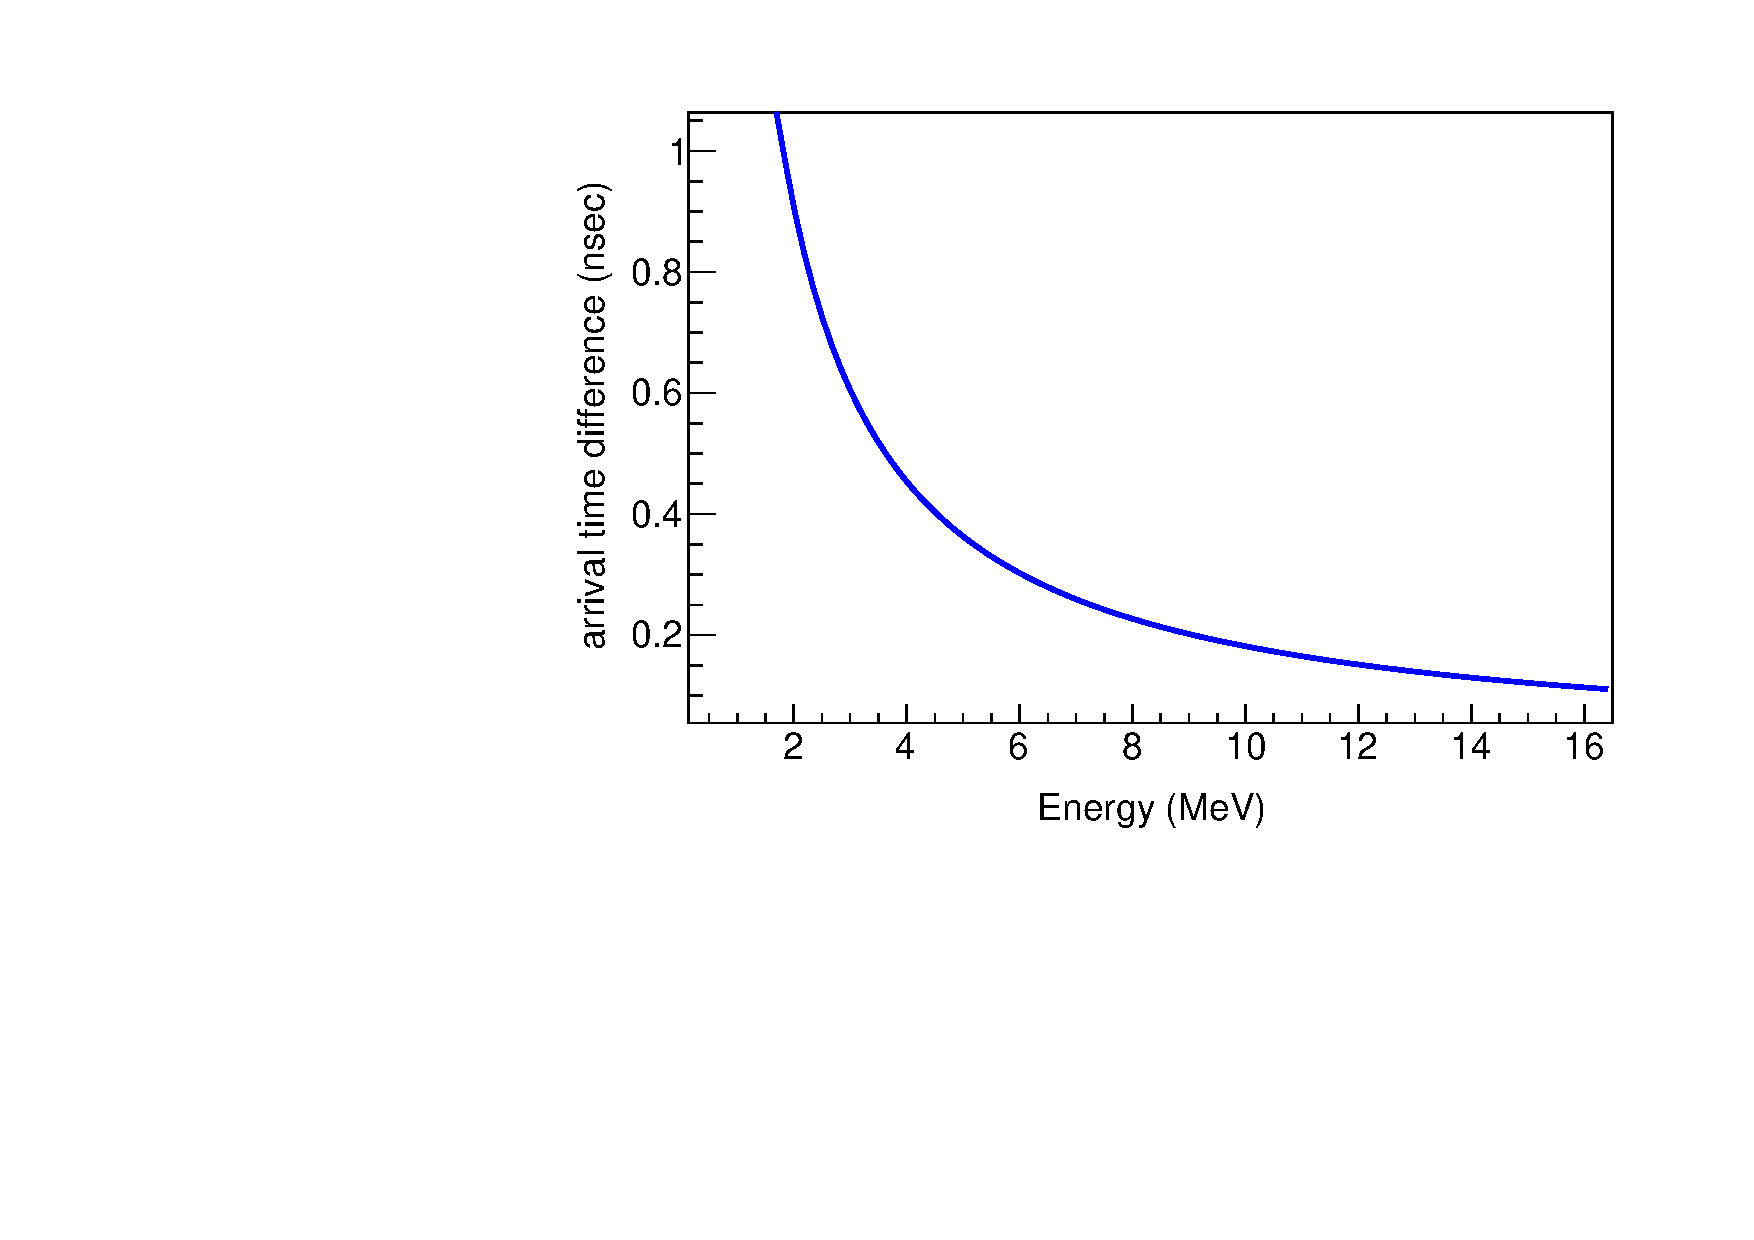
\includegraphics[width=0.5\linewidth]{Figures/deltaTvsE.pdf}} \\
 \includegraphics[width=0.49\linewidth]{Figures/parentEvsdT.pdf} &
 \includegraphics[width=0.49\linewidth]{Figures/nuEvsdT.pdf} \\
			\end{tabular}
%           	\begin{tabular}{c c}
%           	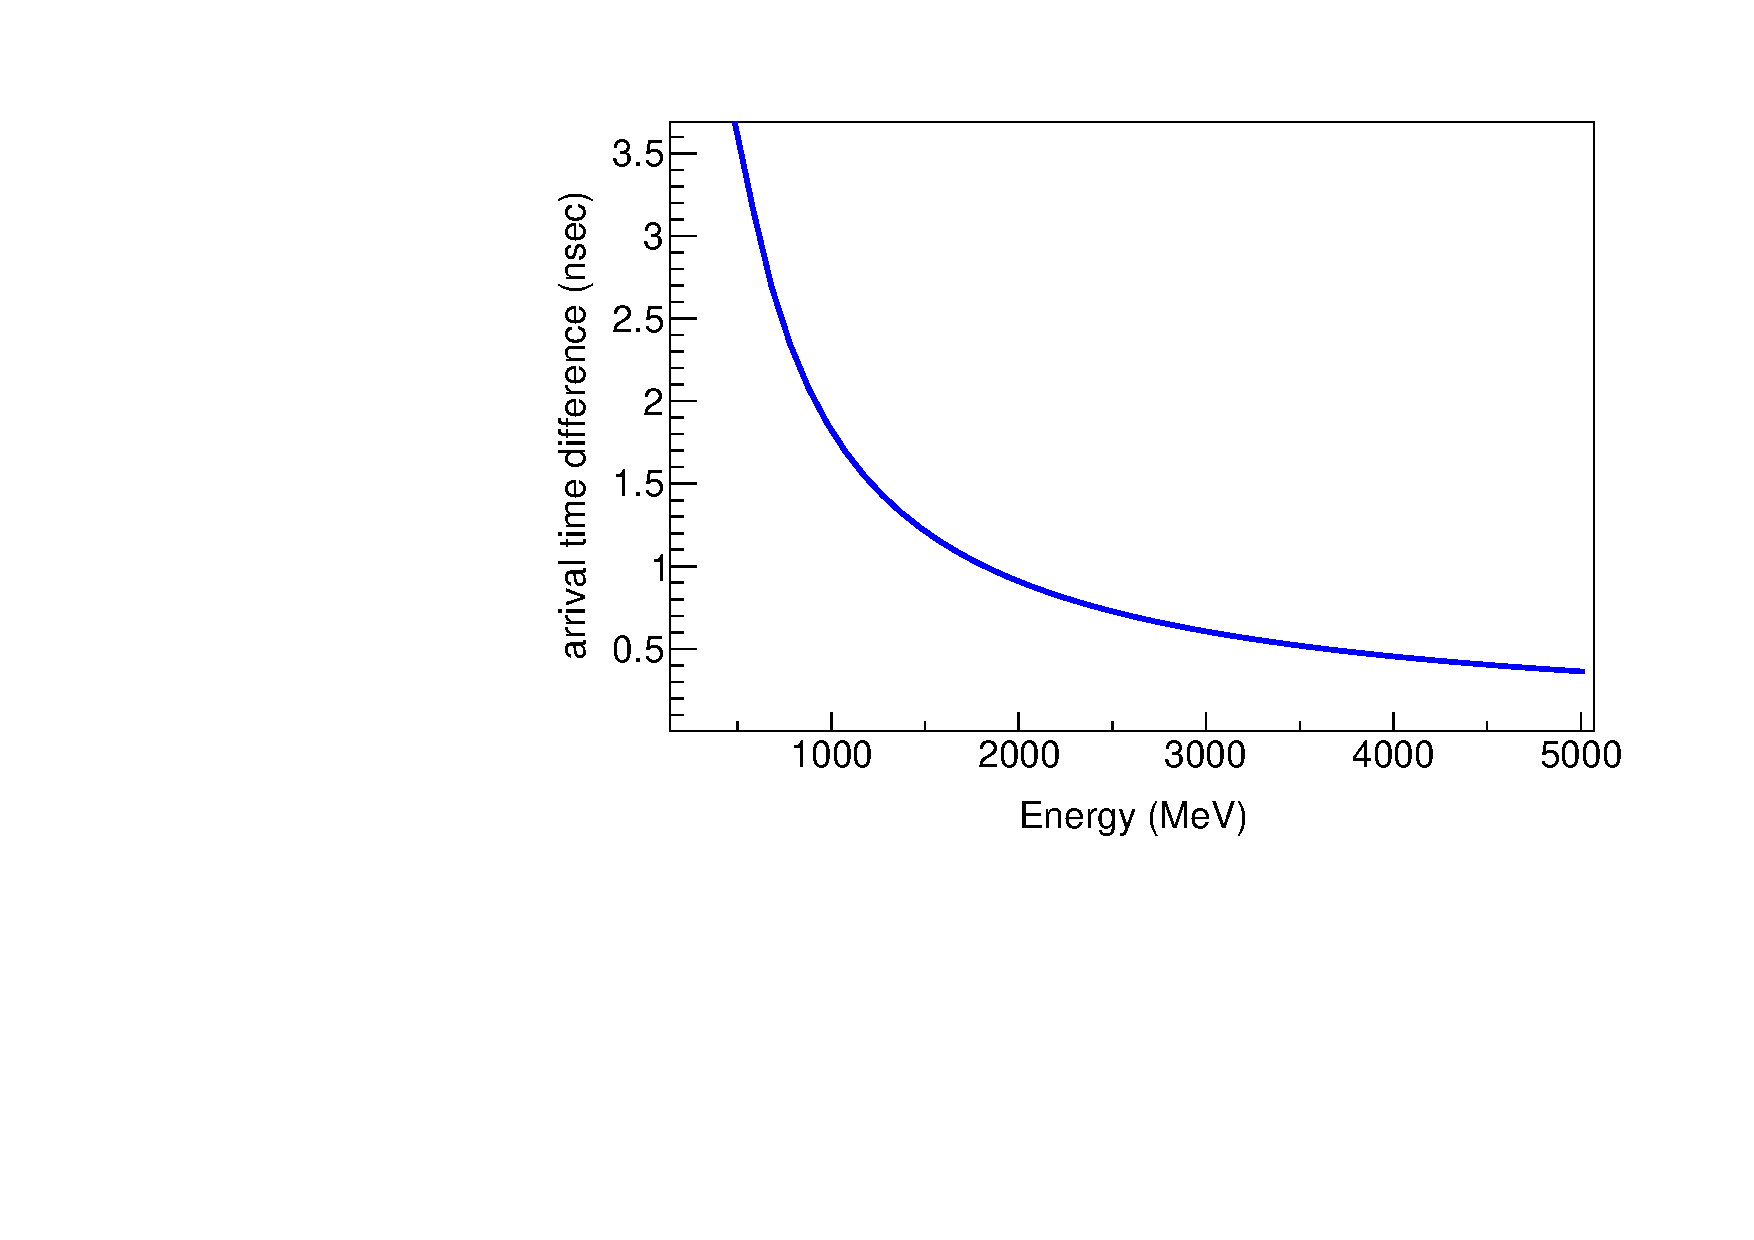
\includegraphics[width=0.455
%                  \linewidth]{Figures/2018.12.3_kinematics/deltaTvsE.pdf}
%                & \includegraphics[width=0.49
%                  \linewidth]{Figures/2018.10.14_LBNFtiming/parentEvsdT.pdf}
%                \\ \multicolumn{2}{c}{\includegraphics[width=0.5
%                    \linewidth]{Figures/2018.10.14_LBNFtiming/nuEvsdT.pdf}}
%			\end{tabular}
	\end{center}
	\caption{Top: A plot of the peak time difference between the arrival of neutrinos from a sub-relativistic pion of energy E' with respect to a relativistic pion (Eq~\ref{eq:beamkinematicsandtiming}). Bottom Left: The simulated relationship between the arrival times and pion energies, for a population of pions produced at the same time. Bottom Right: The equivalents plot of arrival time difference for different energies of the neutrinos.}
		\label{fig:beamkinematicsandtiming}
\end{figure}


\subsection{Achieving Sufficiently Short Proton Bunch Size}
\label{protonbunchsize}

The differentiation of pion energies based on the neutrino arrival time spectrum is tightly peaked in time, with a broad tail. This timing affect is smeared out by the time spread of the proton bunch impinging on the target. Fig~ref{} shows the affect of different proton bunch widths on... At the roughly 1 nsec bunch widths typical of the Fermilab neutrino facilities the correlation between timing and energy is mostly washed out except for a small, low-statistics tail. Bunch sizes of roughly 100 psec would largely preserve the time-energy structure of the beam. Fully exploiting the stroboscopic techniques in the paper would require much shorter bunch sizes, approaching 100 psec. Compressing the existing bunch structure in time is technically feasible do to phase-space limitations among other considerations.

Fortunately, it is possible to rebunch the beam, superimposing a higher frequency substructure. With conventional RF technology one could adiabatically change the beam from $\sim$1 nsec bunches spaced every 100 nsec into $\sim$100 psec bunches spaced by 10 nsec. This structure would simultaneously yield bunches that are both short enough and widely spaced enough to capture the energy and flavor affects. 

In the following sections, we will outline the technical steps...

 


% End Section 2
